\chapter{Planning}


%TODO: Add normal Definition here
\begin{definition} Markov decision process is formalized as a tuple $<S, A, P, R>$, where
\begin{itemize}{}
\item $S$ is a finite set of states of the environment.
\item $A$ is a finite of actions.
\item The transition function $P:S \times A \times S \rightarrow [0, 1]$ defines a probability distribution over the possible next states. 
\item The reward function $R:S \times A \rightarrow \mathbb{R}$ defines the reward after executing a certain action at a certain state.
\end{itemize}
\end{definition}

Given a state of the environment, a policy $\pi: S \times A)$ tells what action should be performed. 
The value function $V^{\pi}: S \times \mathbb{R}$ is the expected cumulative reward when executing
policy $\pi$ from state $s$.

The value function satisfies the Bellman equation:
\begin{equation}
    V^{\pi}(s) = \sum_{s'}P(s'|s, \pi(s))[R(s, \pi(s)) + \gamma V^{\pi}(s')],
\end{equation}
where $\gamma \cin [0, 1]$ is the discount factor which discounts the future reward to the present value.

Similarly, we define the action-value function (or Q function) as:
\begin{equation}
    Q^{\pi}(s, a) = \sum_{s'}P(s'|s, \pi(s))[R(s, \pi(s)) + \gamma Q^{\pi}(s', \pi(s'))].
\end{equation}
The Q function is the expected cumulative reward after executing action $a$ at state $s$ and following
$\pi$ thereafter.

Now lets us extends action set $A$ to include composite actions.

We also need to explicit model the time limit for a composite action to execute, since it
is possible for a composite action to have unachievable terminal state (why?). We do not want 
to wait for the composite action to infinity.

The transition function $P$ and $R$ are modified to include the time limit $t$:
\begin{equation}
    P(s'|s, a, t) = \sum^t_{k=1} \gamma^k Pr(k, s'|s, a),
    \ref{eq:multiProb}
\end{equation}
\begin{equation}
    R(s, a, t) = \sum^t_{k=0} \gamma^k r_k,
\end{equation}
The value function needs to be modified as:
\begin{equation}
    V^{\pi}(s) = \sum_{s'}P(s'|s, \pi(s), t)[R(s, \pi(s), t) + \gamma^N V^{\pi}(s')],
\end{equation}
where $N$ is the number of steps for the action $\pi(s)$ to finish its execution.
A question arises since we do not know the actual time to finish executing each composite action.
Let's set $gamma=1$ from now on.
%TODO: (how MaxQ solve it?).

Although the state abstraction provides us compact state representation, 
it doesn't change the size of the planning envelope. Thus we do not gain any computational
advantage by applying such an abstraction technique.

A key observation of this work is to adopt an unsafe projection function. 
The size of planning envelope grows exponentially with the number of features.
By assuming 
some features do not change during the execution of actions, we do gain computational advantage by
significantly reducing the size of the planning envelope. 
We lose the optimally with this approximation technique, but it is necessary because we want 
to apply our work beyond toy applications.
Our approach doesn't imply that
part of the features are completely ignored. The agent still computes the plan according to 
the new value of t)e features.
Besides, the model-free layer still operates with the full observation of the state. 
If we put more features into the model-based layer, we would get a more precise plan at the cost
of more samples required to estimate the model parameter and more time spent on computing the plan.
Therefore, the number of features included in the model-based layer depends on the available 
computation resources.
The objective of our work is not to show how to find the optimal arrangement of features, but to indicate
that there is a trade-off between model-based and model-free approaches.
By adjusting the arrangement of features, we can maximize the performance of the agent without exceeding
the capacity of available computational resources.
%TODO: the grid world example--> assuming monster does not move is correct
%TODO: show that approximation is necessary--> the planning envelope is exponentially huge wrt the number of monsters

To compensate the incapability to predict the movement of the monsters in the long run, 
we exploits the model-free approach to handle the dynamic of the environment in the short period.
The choice

\section{Estimation of the transition probability}

Each model-based layer (except the top one) needs to compute the state transition probability
from the given state $s$ to some terminal state $x$.
\begin{equation}
    P(x|s) = max_a P(x|s, a).
\end{equation}
\begin{equation}
    P(x|s, a) = P() from all other states
\end{equation}
It can be done by querying the transition probability from the child layers.
Same for the reward.

Each model-free layer with a parent model-based layer also needs to compute the transition probability.
Since the child layers of model-free layer do not provide such information, the model-free layer
needs to estimate the probability based on its current policy.

\begin{figure}[h]
    \centering
    \begin{minipage}[t]{0.6\linewidth}
        \centering
        \includegraphics[width=\textwidth] {./figures/monsterPlan.eps}
    \end{minipage}
    \caption{The shortest path from the agent's location to the food}
    \label{fig:MonsterPlan}
\end{figure}

Take the eat-food-and-avoid-monster game in Fig. \ref{fig:MonsterPlan} as the motivating example. 
The top level planner finds a path to the location of food. 
The low level deals with primitive actions to go the destination specified by the top level planner.
If the monsters do not move and the actions are deterministic
, the optimal policy of the game can be founded by the shortest path algorithm. The goal state is the location of the food,
the cost to move to the adjacent location is $1$, if there is a monster in the adjacent location, the cost 
to move to it is $\infty$. The agent only needs to compute the lowest cost path from its current position to the goal,
and choose the action which can keep it on this precomputed path.

However, the game is not a static one. The monsters may move around and block the precomputed path. The actions of
agent may have unpredictable result to lead it out of the precomputed path.
%This stochastic natural of the game makes it natural to formulate the problem as a stochastic shortest path
%problem. A stochastic shortest-path (SSP) problem is a MDP problem with a absorbing goal state and positive costs.
%A solution of a SSP problem is a policy from the initial state to the goal state with minimum expected cost.

A work by Zucker et al. \cite{Planner} introduced a two-level approach to solve a maze problem.
The planner uses the shortest path algorithm to find a path from the current state to the goal state.
The cost of each step is estimated by Q value, which is computed by the SARSA algorithm.

A issue occurred when we want to apply this approach to general MDP problems: we do not know the 
goal state. The objective of MDP is to find a sequence of actions which can maximize the overall 
rewards. There are no clearly defined "goal" for the MDP problems.

A possible way to adopt the planning technique to the MDP problems is to choose a sequence 
of goals which can maximize the overall rewards. The goal can be chosen to be the state
with the highest expected reward. To achieve this, an agent needs to learn 
the probability to move from one state to another, and the reward to be received
from each state. 

The approach is two fold. In the beginning, the planner selects a path from the current 
state to the goal state with the highest expected reward. The path consists of several
nodes, which are considered as the subgoals of the plan. The RL agent finds the subgoal 
right after the current state, and chooses a sequence of actions which can lead the agent
to the subgoal. The result can be either success or failure, and the probability of the successful
rate of a plan would be updated accordingly. The planner then use the updated information to 
compute a new path.

%\section{The task hierarchy of eat-food-and-avoid-monster game}
%\section{Training the RL agent}
The training is done in $5 \times 5$ with one food and one monster.
A goal is assigned to the agent at the beginning of the episode. 
The goal is the desired next position of the agent.
%The goal is the position difference of 
%the current position and the next position. It can be either $(0, 1), (0, -1), 
%(1, 0) or (-1, 0)$.
The action of the agent terminates after 1 step regardless if the agent achieves the goal 
or not. The task of the RL agent is to find an optimal policy to achieve the goal. 
Although the optimal policy is obviously corresponding to the four primitive actions (north, south, west or east) 
, the agent doesn't have any prior knowledge of it. Moreover, the agent should not always comply to the indication of the goal.
If the goal asks the agent to go north but there is a monster at north of the agent, it is unwise to go north to achieve the goal.

To construct a RL agent which may follow the instruction of the planner when possible, 
we give the reward of the RL agent $+20$ when it achieves the goal and $0$ otherwise.
If the agent gets into a monster, it receives $-30$ reward as usual.

The planner makes the plan based on the state transition probability and the corresponding reward for each transition.
The RL agent needs to provides such an information to the planner (note that the state transition probability and the reward
depends on the current RL agent policy).
The information must be learned as well. 
The reward given by the planner (like the reward for achieving the goal) is called internal reward.
The internal reward is constructed to get the desired behavior of the RL agent.

The reward given by the game itself is called external reward.  It is what the
planner tries to maximize. The expected external reward for the agent to move
from current state $s$ to the goal state $g$ within $t$ steps is:

\begin{equation}
    R_{E}(g, s, t) = Q_{E}^{g, t}(s, \pi(s)), 
\end{equation}
where $\pi$ is the policy of the RL agent which directs it agent to go to the goal state within $t$ steps.
$\pi(s)$ is one of the primitive actions.
$Q_{E}$ is the expected external reward function for the agent to get at state $s$ if 
the RL agent takes action $\pi(s)$.

The RL agent estimates the $Q_{E}$ by SARSA algorithm -- after the RL agent takes the action $a$
and observes next state $s'$, reward $r$ and next action $a'$, the $Q_{E}$ is updated by:
\begin{equation}
    Q_{E}^{g, t}(s, a) \leftarrow  Q_{E}^{g, t}(s, a) + \alpha [r + \gamma Q_{E}^{g, t-1}(s', a') - Q_{E}^{g, t}(s, a)]
\end{equation}

The RL agent estimates the probability to achieve the goal by the same equation:
\begin{equation}
    P^{g, t}(s, a) \leftarrow  P^{g, t}(s, a) + \alpha [\delta + \gamma P^{g, t-1}(s', a') - P^{g, t}(s, a)]
\end{equation}

$\delta$ is 1 when the RL agent achieves the goal state (if $s'$ is the goal state) and 0 otherwise.

The policy $\pi(s)$ of the RL agent is determined by the expected internal reward function $Q_{I}$.
\begin{equation}
    \pi(s) = argmax_a Q_{I}^{g, t}(s, a), 
\end{equation}
Similarly, $Q_{I}$ can be estimated by SARSA algorithm.

\begin{figure}[h]
    \centering
    \begin{minipage}[t]{0.9\linewidth}
        \centering
        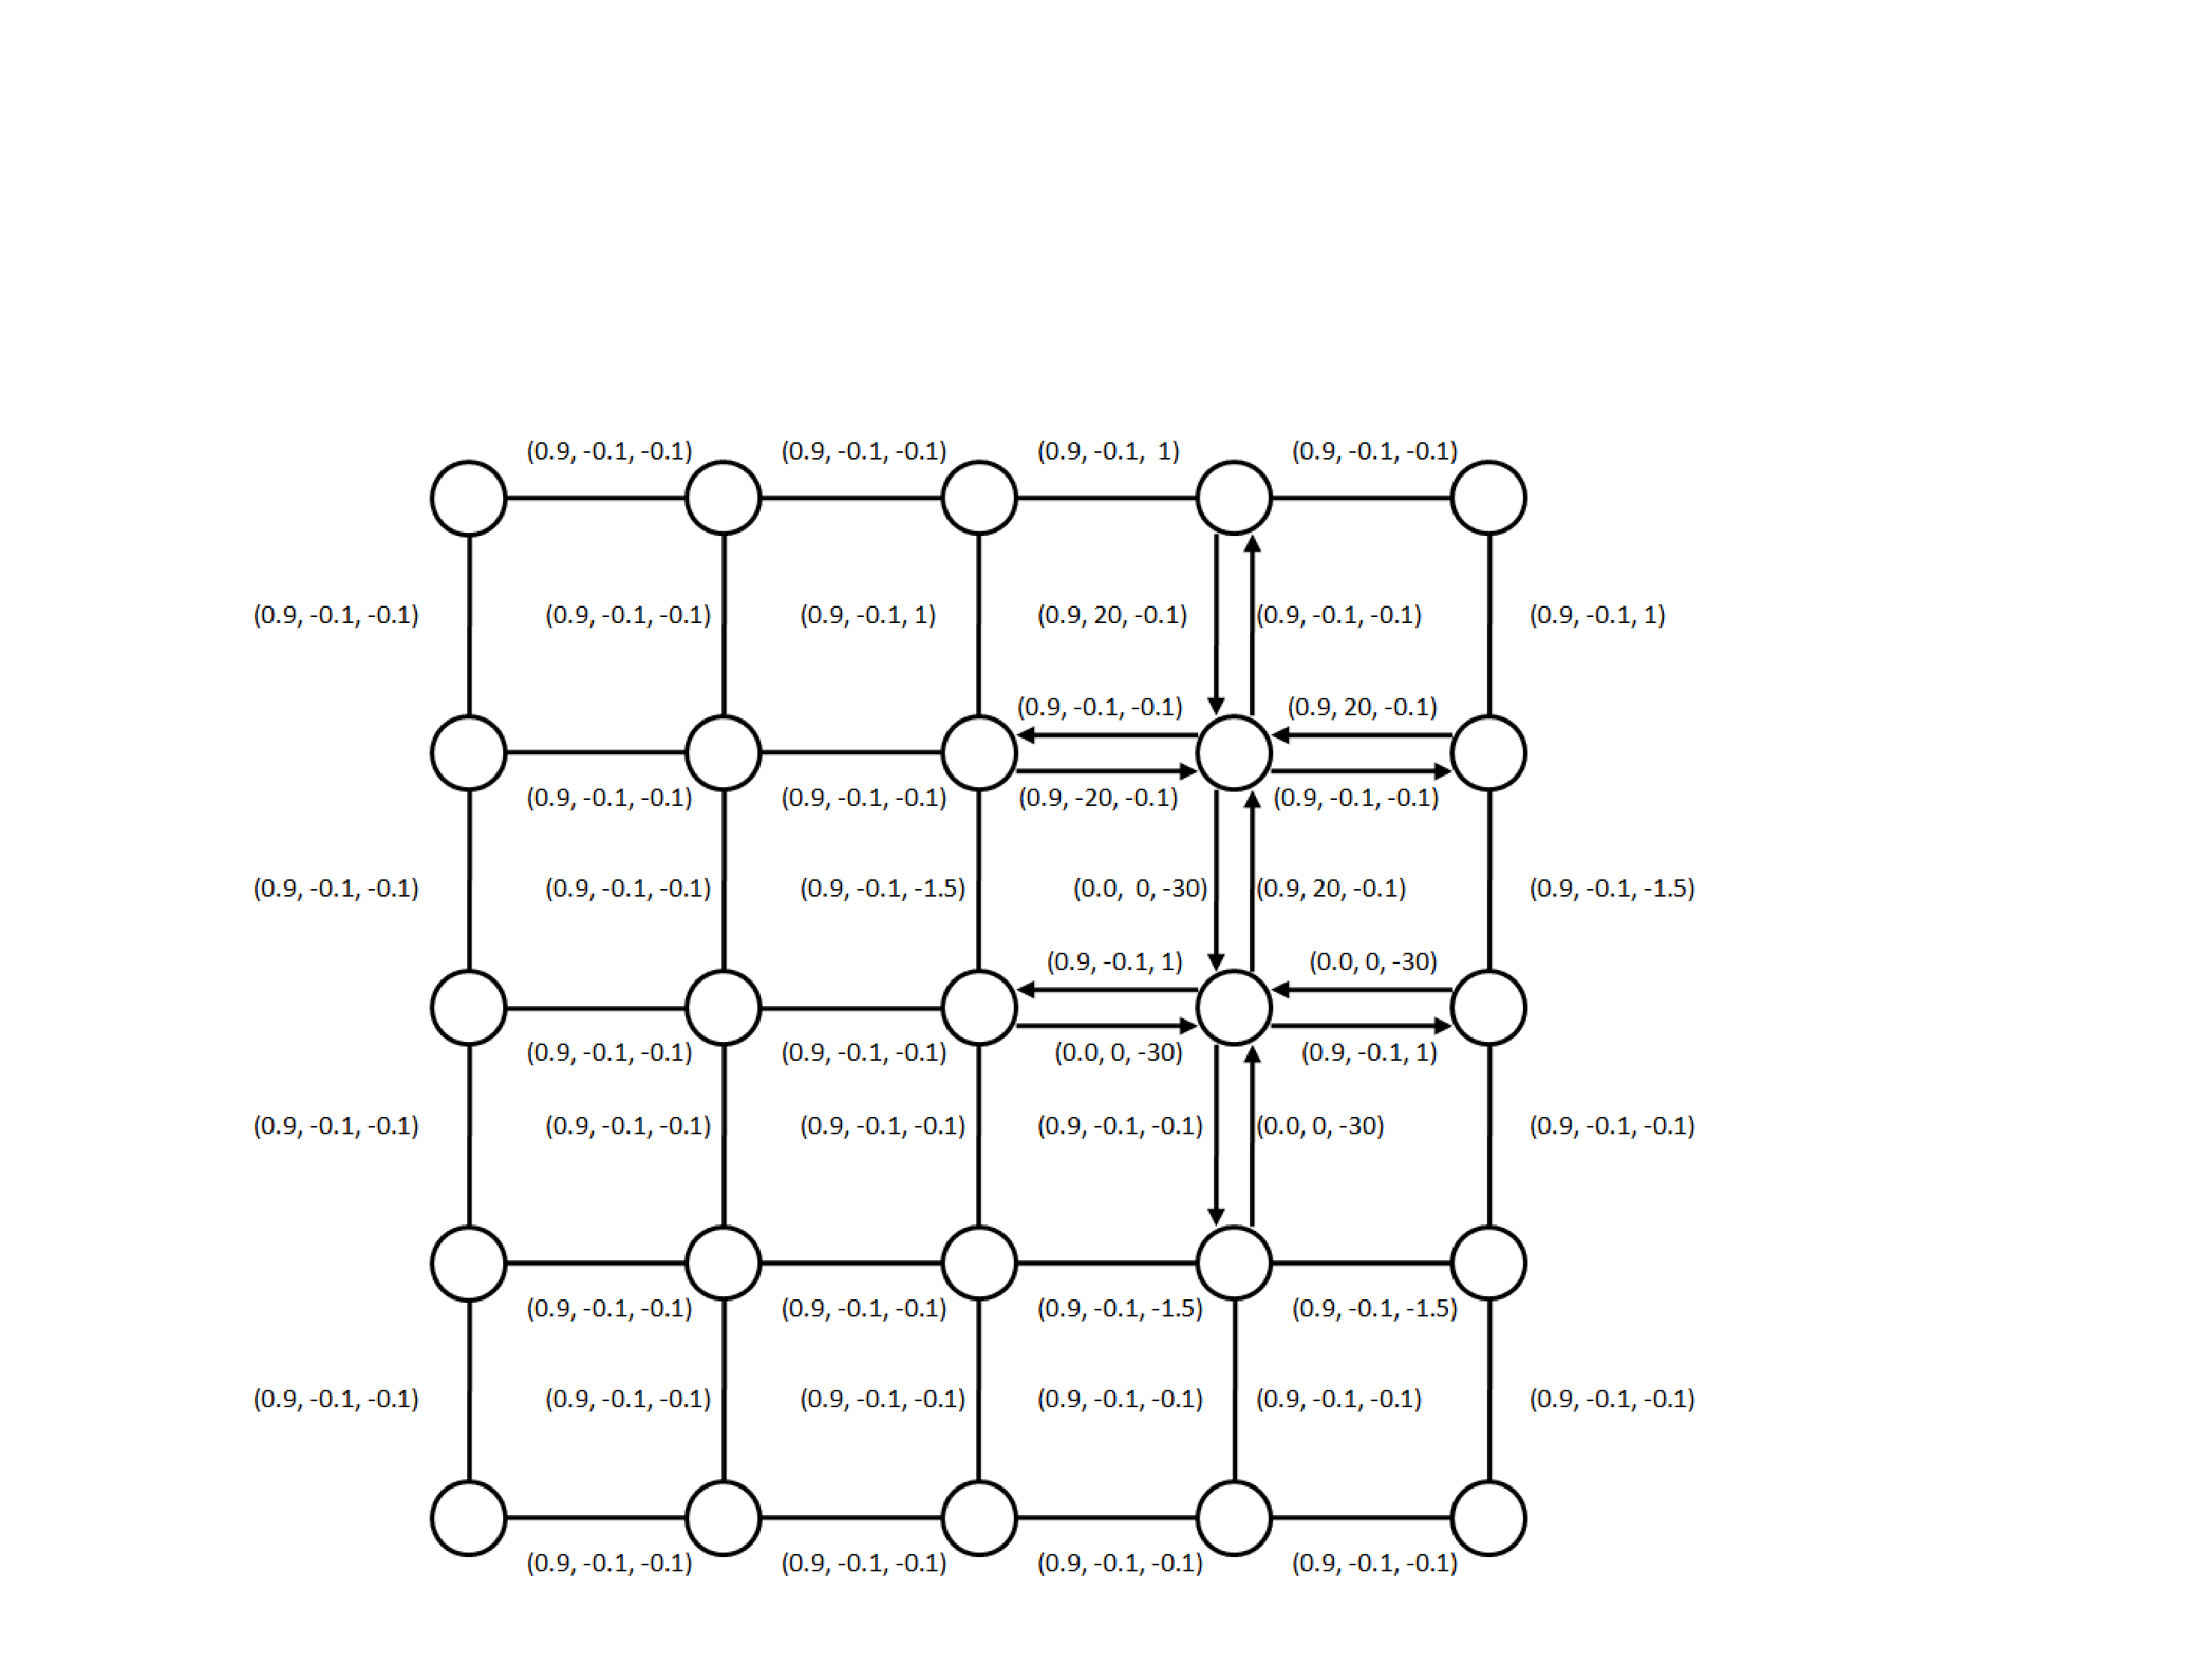
\includegraphics[width=\textwidth] {./figures/PlanGraph.eps}
    \end{minipage}
    \caption{The transition probability and reward for the game in Fig. \ref{fig:MonsterPlan}}
    \label{fig:PlanGraph}
\end{figure}

To construct a plan, the planner uses shortest-path algorithm to find a path with maximum expected reward.
For example, the plan in Fig. \ref{fig:MonsterPlan} corresponding to the expected reward of 
$18*0.9^5$ with the estimated transition probability and)reward shown in Fig. \ref{fig:PlanGraph}.
In general, the expected reward of the plan $p = (s_1, s_2, \dots, s_n)$ can be computed by: 
\begin{equation}
    R_P(p) = R_E(s_2, s_1, t) + R_E(s_3, s_2, t)P^{s_2, t}(s1, \pi(s1)) + \dots + R_E(s_n, s_{n-1}, t)P^{s_n, t}(s_{n-1}, \pi(s_{n-1})) \dots P^{s_2, t}(s1, \pi(s1))
\end{equation}



\endinput
%Most of the previous work on RL focus on model-free approaches for several reasons. 
%The most 
%Within a planning agent, there are at least two roles for real experience: it
%can be used to improve the model (to make it more accurately match the real
%environment) and it can be used to directly improve the value function and
%policy using the kinds of reinforcement learning methods we have discussed in
%previous chapters. The former we call model-learning, and the latter we call
%direct reinforcement learning (direct RL). The possible relationships between
%experience, model, values, and policy are summarized in Figure  9.2. Each arrow
%shows a relationship of influence and presumed improvement. Note how experience
%can improve value and policy functions either directly or indirectly via the
%model. It is the latter, which is sometimes called indirect reinforcement
%learning, that is involved in planning. 

%The second branch is model-based RL, which directly estimates
%a model of the environment and then plans with
%this model. Early work demonstrated that summarizing an
%agent’s experience into a model could be an efficient way
%to reuse data (Moore & Atkeson, 1993), and later work utilized
%the uncertainty in an agent’s model to guide exploration,
%yielding the first (probabilistic) finite bounds on the amount of data required
%to learn near-optimal behaviors in the general case (Kearns & Singh, 1998;
%Kakade, 2003).


%motivation: play a randomly generate maze to adapt to
%adapt to noval situation

%weakness-> an adversary to block the path forever
%no knowledge (coin won't disappear-->need hack to do it, moster won't move)
%comparison to the previous work->HRL,


%model based-> state space is too large. good to train with
%few examples (10 sec training)
%model free-> cannot handle randomly generated maze -> failed to adapt to noval situation. can handle large space (linear SARSA)
%Experiment: comparison with flat model based approach and hierarchical model based approach with approximation

%combine both-> use model based on top level to reduce
%the state space, and model free on bottom to 
%deal with randomized noisy world for short term reward

%build multilevel of hierachy on features
%label each room with a number 1, 2, 3
%the coordinate of wrt the room
%(1, (25, 30))
%move from room 1 to room 2
%top level
%action (1->2)
%second level
%assume (1, (25, 30)) -> (2, (0, 0))
%action ((25, 30) -> (0, 0)) goal (-25, -30) in single step

%need to build time model of the full state
%P(s->s'|x, t) the propability to move from state s to s'
%after t steps of the observation of full state x

%power coms from trasition model (model the shortest path), not shortest path
%you can use model-based approach on this

%fickle passenger of MaxQ
%coarseness on time and space scale

%-->you can work on continus varible now, no more grid world

%1. Assumption on the state difference (if it is not true --> like the agent in a world boundary or the health is 100 and cannot be imporve
  %since the state is outside the known state boundary, the planner whon't plan for it. but the local planner may still direct the agent
  %to go outside the world boundary, which may be a problem)
%2. Application to the hierachical RL
%3. Limitation: unachievable state (a coin surrounded by many monsters)
%4. Can inference in a very small world, not need to do 64 by 64
%Sometimes we need a plan. The greedy approach of reinforcement learning does not always work. 
%RL techniques have several limitations:
%1. It's difficult for to transfer the value function from a small world to a large one. If the agent has
%the experience only in a small world like 4 \times 4 grid, it cannot act well in 64 \times 64 grid
%because it does not know the correct action in regard to an object 63 grid away.

%2. It takes a long time to train the agent to be good enough. The greedy 

%3. The approximation only good in a small range. We need a plan for long term action.
%The noval state (the state in current game which has not been experienced) may 

%4. Impossible task to maze problems: RL require that optimal agent to find the optimal solution for a maze when all the features
%are input to the agent. Which is unlikely to work.(impractical when the maze is large)(unable to transfer
%the knowledge from previous maze experience to the current one) A practical solver shall invovle planning through 
%the possible route and find the one which can lead to the exist.
%All the work requires the agent to repeat play the same maze (assuming traps) until it finds the optimal solution.
%What if the maze changes every time?

%1. Is it guarranteed convergence? Yes, if we choose the goal next to the current state which leads to highest Q value. 
%It is the same as SARSA.
%2. How to choose the goal to guarrante convergence to optimal policy?

%Good to work on the problem with a long term reinforcement (feedback) like a maze.
%Bad to work with a problem with dynamic envirment (everything changes with or without agents actions)
%Bad when the consequence of an action is delayed for many steps. (poison)

%Q: prove that RL cannot solve maze problem
%Ability to transfer the knowledge from one maze to another
%compare the HRL in key-finding problem
%compare to the model-based RL





%application: the key-room problem--> each room lock a key, one room has a treasure, the agent needs to go through 
%a maze to collect the keys for each door and get the treasure

%Stochastic Shortest-Path Problems
%A Stochastic Shortest-Path problem is an mdp prob-
%lem in which the state space S = f1; : : : ; n; tg is such
%that t is a goal (target) state that is absorbing (i.e.,
%p(t; u; t) = 1 and g(t; u) = 0 for all u 2 U(t)), and the
%discount factor ® = 1. In this case, the existence of
%optimal policies (and optimal stationary policies) is a
%major mathematical problem. However, the existence
%is guarantee under the following reasonable conditions:
%(A1) There exists a policy that achieves the goal with
%probability 1 from any starting state.
%(A2) All costs are positive.
%The ¯rst assumption just expresses the fact that the
%problem admits a well-behaved solution. Such policies
%are known as proper policies. The second assumption,
%in the other hand, guarantees that all improper policies
%incurs in in¯nite cost for at least one state. Thus, both
%assumptions preclude cases where the optimal solution
%might \wander" around without never getting to the
%goal. For example, a problem having a zero-cost cycle
%(in state space) violates the second assumption.
%As mentioned in the Introduction, often we are only
%interested in knowing how to go from a ¯xed initial
%state, say 1, to the goal state. The optimal solution in
%this case is an partial optimal stationary policy ¹ such
%that ¹(i) = ¹¤(i) for all states i that are reachable
%from 1 when using the optimal policy ¹¤; the so-called
%relevant states when starting from 1.1
%Finding a partial optimal policy can be consider-
%ably simpler, the extreme case when the set of relevant
%states is ¯nite and the complete state space is in¯nite.
%Thus, the question of how to ¯nd partial optimal poli-
%cies is of great relevance. One algorithm for that is
%Real-Time Dynamic Programming.

%There are two ways for a RL agent to use its sample data. It can use the sample data to update the 
%value function and improve its policy. It is called model-free (or direct) reinforcement learning. 
%Another approach is to use the sample data to estimate parameters for the model of the environment and compute the value function
%from the model. It is called model-based (indirect) reinforcement learning.

%The advantage of model-based approaches is that they make more efficient use of the sample data, thus 
%it take fewer time to train a model-based RL agent. Other the other hand, model-free approaches do not assume 
%a prior model, so it would not be affected by the bias of the model design. Besides, the existence of 
%good linear approximation algorithms, such as linear SARSA, makes it possible for model-free approaches to
%handle large scale problems.

%Model-based approaches needs to enumerate through all possible states to compute the value function. 
%But the number of states grows exponentially with the number of features, 
%and it quickly becomes intractable if the number features grows large.

%The main idea of this work is to combine the model-free, model-based and hierarchical reinforcement learning.
%For the lower level of hierarchy, we adopt the model-free approach to handle the complete and possibly large state space.
%On the top level of hierarchy, we use the model-based to plan on a coarser level, which contains only small number of states.
%This approach allows the agent to plan on the higher level and make efficient use of the sample data. On the lower level,
%the agent uses model-free approaches with linear approximation to handle the complete state space.

%The prior works on hierarchical reinforcement learning (HRL) can be divided into two categories: model-free and model-based approaches. 
%The model-free approaches include HAMQ \cite{HAMQ}, MAXQ \cite{MAXQ}, SMDP and options framework \cite{option}
%For model-based approaches, Seri et al. \cite{HLearning} proposed a model-based HRL in average reward setting.
%Diuk et al. \cite{Diuk} adopted model-based HRL to deterministic domain. Jong and Stone \cite{RMaxQ} combined 
%R-MAXQ and MAXQ to achieve efficient model-based exploration and the action abstraction of MAXQ.
